\documentclass[a4paper, fleqn]{article}

\usepackage{amsmath}
\usepackage{enumitem}
\usepackage{graphicx}
\usepackage[style=alphabetic]{biblatex}

\begin{document}

\title{Capstone I - Journal 03 \\ Project 61 $\cdot$  Steelcase \\ Reduction of Logistics and Packaging Costs}
\author{Basil R. Yap}
\date{2018 March 19}
\maketitle

\section{Summary}

\textbf{Predictions and outline given in prior Journal\footnote{Journal 02}:}\begin{itemize}
\item \textbf{Week 7:} Site visit \& data cleaning
\item \textbf{Week 8:} Load optimization modelling
\item \textbf{Week 9:} Model implementation
\end{itemize}
Given the information collected during the site visit, I have re-evaluated the importance of load optimization in the earlier stages of ideation and redoubled my efforts to helping ideate for possible improvements for SMM's\footnote{Steelcase Manufacturing Malaysia} current package solution.\\
\vspace{1pt}\\
With a greater insight of the actual manufacturing process of the three mechanism components we want to focus on, I believed it was more prudent to ideate for potential solutions as soon as possible, while the memory of our visit was still fresh. Given this shift in focus, the planned outline of the week 8 \& 9 were changed to the following:\begin{itemize}
\item \textbf{Week 8:} Breadth oriented ideation
\item \textbf{Week 9 (Proposed):} Feasibility analysis
\item \textbf{Week 9 (Actual):} Formalisation of problem scope
\end{itemize}
The overall idea was to have the group independently generate as many diverging ideas as possible. Then, slowly over the span of weeks prune the number of ideas down to manageable enough amount for deeper investigations into each respective idea.\\
\pagebreak
\section{Problems Encountered}
\subsection{Week 7 \& 8}
During the site visit, the manufacturing process was extensively documented from assembly of the mechanisms to the loading of the packages. Various factors/variables were identified to be key to the design of our future solution. In the order of process stage, the problems are as follows:\begin{itemize}
\item \textbf{Folding of packaging:}\begin{itemize}
\item Packaging is not pre-folded and components need to be stored in an accessible storage compartment
\item The boxes are highly compartmentalised and consists of many pieces that require assembly 
\item The boxes tend to be quite low, requiring the worker to frequently bend down
\end{itemize}
\item \textbf{Loading of mechanism:}\begin{itemize}
\item Mechanisms are covered with a disposable plastic prior to loading.
\item The method of loading varies widely between the three mechanisms, the complexity of how it is loaded must be taken into consideration.
\item The assembly cycle time varies widely between the three mechanisms, the loading step is a bottleneck in some cycles.
\item Depending on the weight of the mechanism, the boxes used were required to be double or triple layered in order to ensure its integrity while in transit
\item The pallets used for the packaging of all three mechanisms are the same, therefore, the footprint of every box is identical with varying heights. This constraint severely affects the packing efficiency of the V2 mechanism.
\end{itemize}
\item \textbf{Loading of boxes:}\begin{itemize}
\item The number of boxes that can be stacked sequentially is limited by a prior load test. With the current paper pallets, The maximum number of each stack is 3 boxes high.
\item The loading of the mechanism boxes are done purely by forklifts, which are accurate enough to position the boxes with minimal gaps.
\item The compartmentalisation of the mechanisms and the usage of the disposable plastic is to ensure that the mechanisms do not scratch or gather dust.
\end{itemize}
\end{itemize}
\pagebreak
\subsection{Week 9}
Due to an oversight on my part, the problem scope of our project was reduced too significantly with the complete removal of the logistics management\footnote{In-depth explanation regarding its removal is available in Journal 02} component of the project. In addition to that, the entirety of the problem scope was not well documented nor formalised prior to the completion of Review I. Week 9 was, therefore, spent on documenting the problem scope thoroughly and to build up a case for the re-introduction of the logistics management component and the data needed to sustain the problem. During this period, I focussed predominantly on building up the logistics management case and its incorporation into our current problem scope.


\section{Actions Taken}

Based on the information gathered from the site visit, the direction I believed to be the most fruitful was to redesign the external dimensions of the box, or at the very least, find a pallet size which would allow for all three mechanisms to have minimal space wastage. During week 8, my ideation and research efforts centred around finding literature and industry best practices for designing efficient packaging solutions. This knowledge was also supplemented literature on spatial packing optimization.\\
\vspace{1pt}\\
The list of readings, I compiled are as follows: \\\textit{texts in italics, were of particular significance}\begin{itemize}
\item \textbf{3D packing optimization:}\begin{itemize}
\item \textit{Mathematical model and efficient algorithms for object packing problem}\\\textit{N Chernov, Y Stoyan, T Romanova}
\item The 3D-Packing by Meta Data Structure and Packing Heuristics\\
H Yamazaki, K Sakanushi, S Nakatake
\item A packing algorithm for particles of arbitrary shapes\\
X Jia, RA Williams
\end{itemize}
\item \textbf{Package design:}\begin{itemize}
\item \textit{Structural Packaging}\\
\textit{P Jackson}
\item Package Design Workbook: The Art and Science of Successful Packaging\\
S DuPuls
\end{itemize}
\end{itemize}
\pagebreak
\section{Insights Obtained}

\subsection{3D packing problem} \cite{1}
\textbf{Why do we need to optimize a simple block fitting problem?}\\
Optimizing for a 3D packing problem allows the team to consider non-conventional box shapes. i.e. non-cuboid shaped boxes\\
\vspace{1pt}\\
A 3D packing problem is equivalent to a 3-dimensional cutting and packing problem, where instead of extracting 2D shapes from a 2D board, we are attempting to extract 3D composite polygons (\textit{packages}) from a 3D container (\textit{container}). In Figure \ref{figure:2d3d}, an extreme case of 3D packing problem solution is demonstrated.
\begin{figure}[h!]
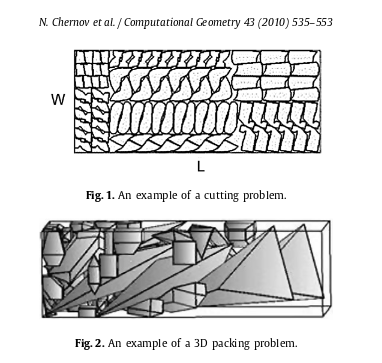
\includegraphics[width=\linewidth]{./assets/201803260707.png}
\caption{2D/3D cutting and packing problems}
\label{figure:2d3d}
\end{figure}
\pagebreak
Given the design of our box, we can breakdown/approximate the shape of the box into a combination of 3D phi objects. Phi objects are mathematical representations of geometrical shapes we can use as variables in our 3D packing problem. In the event our boxes do not conform to a conventional shape, we can derive its phi function as a composite of simpler phi functions such as spheres, cones and cuboids. A example of a composite pi function can be seen in Figure \ref{figure:phifunction}. Using proposed solutions in the paper, we can derive the optimal positions and rotations of each box in the container.
\begin{figure}[h!]
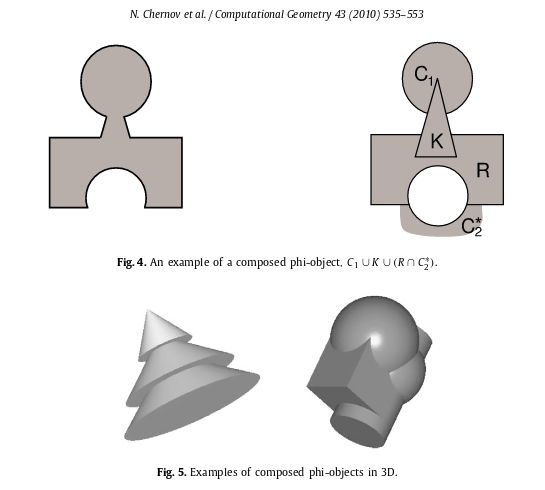
\includegraphics[width=\linewidth]{./assets/201803260719.png}
\caption{2D/3D composite phi functions}
\label{figure:phifunction}
\end{figure}
\pagebreak
\subsection{Package design}\cite{2}

When designing a package box, there are two major design decisions to consider:
\begin{itemize}
\item The net of the volumetric shape
\item The stability of the volumetric shape
\end{itemize}
The net is the unfolded 2D space the volumetric shape occupies. In order to be able to mass produce the boxes, the shape has to be as compact and space efficient as possible. To do so, the author came up with 11 steps to efficiently create the net of most full body shapes. Figure \ref{figure:nets} shows the outcome of following the following steps:
\begin{enumerate}[label=\textbf{Step \arabic*} ]
\item Create 3D form
\item Identify 2D faces
\item Label edges on the faces
\item Cut out lib/top of box
\item Cut out shortest edges
\item Unfold remainder of the box in ascending order of edge length
\item Label lid/top outermost edge with T
\item Label alternating outermost with T and X
\item Ensure all T labelled edges can hold a Tab
\item Determine the shape of each Tab by the shape of the corresponding X-labelled face
\end{enumerate}
\begin{figure}[h!]
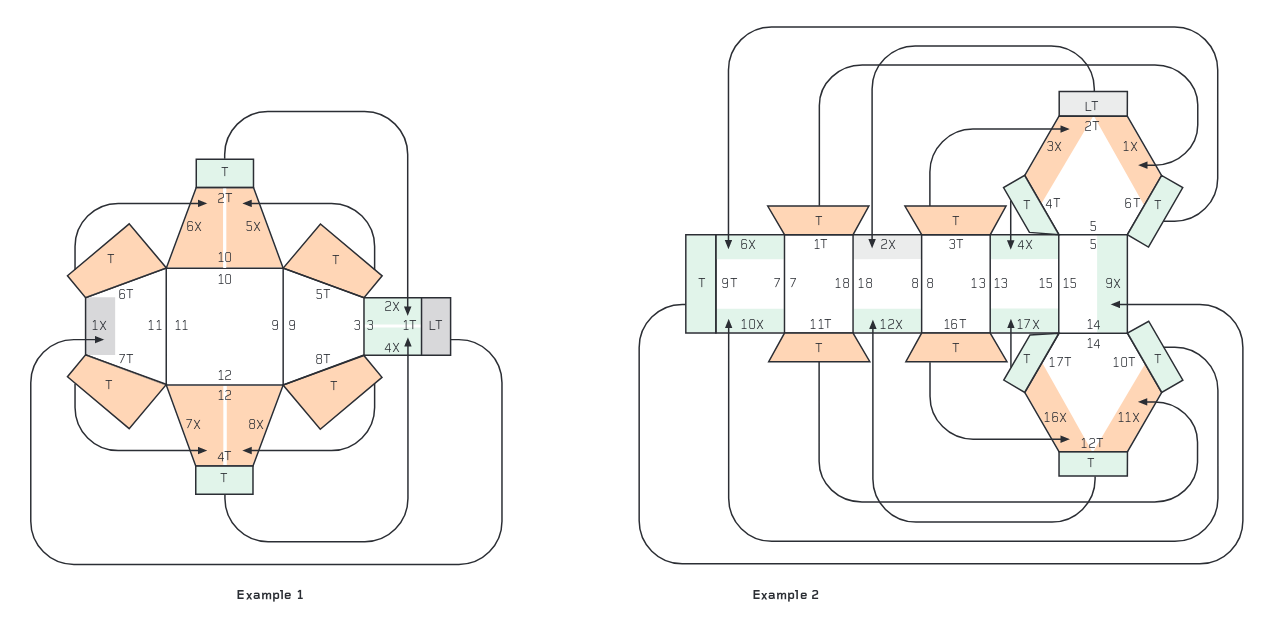
\includegraphics[width=\linewidth]{./assets/201803260810.png}
\caption{Procedurally generated nets}
\label{figure:nets}
\end{figure}
\section{Timeline}

The my personal timeline for next three weeks are as follows:
\begin{itemize}
\item \textbf{Week 10:}    \begin{enumerate}
\item Re-negotiate data and problem scope for logistics management problem
\item Re-scope ESD component (if applicable)
\item Compile ideas from independent ideation for package design
\end{enumerate}
\item \textbf{Week 11:}     \begin{enumerate}
\item Feasibility analysis of ideas
\item ESD component (to  be confirmed)
\end{enumerate}
\item \textbf{Week 9:}    \begin{enumerate}
\item In-depth research on short-listed ideas
\item ESD component (to be confirmed)
\end{enumerate}
\end{itemize}
\begin{thebibliography}{9}
\bibitem{mathpack}
N Chernov, Y Stoyan, T Romanova
\textit{Mathematical model and efficient algorithms for object packing problem}
Computational Geometry, 2010
\bibitem{designpack}
P Jackson
\textit{Structural Packaging}
Laurence King Publishing, 2014
\end{thebibliography}
\end{document}